\documentclass[a4paper,12pt]{article}

%%% Работа с русским языком
\usepackage{cmap}					% поиск в PDF
\usepackage{mathtext} 				% русские буквы в формулах
\usepackage[T2A]{fontenc}			% кодировка
\usepackage[utf8]{inputenc}			% кодировка исходного текста
\usepackage[english,russian]{babel}	% локализация и переносы
\usepackage{comment}


%%% Дополнительная работа с математикой
\usepackage{amsfonts,amssymb,amsthm,mathtools} % AMS
\usepackage{amsmath}
\usepackage{icomma} % "Умная" запятая: $0,2$ --- число, $0, 2$ --- перечисление

%% Номера формул
%\mathtoolsset{showonlyrefs=true} % Показывать номера только у тех формул, на которые есть \eqref{} в тексте.

%% Шрифты
\usepackage{euscript}	 % Шрифт Евклид
\usepackage{mathrsfs} % Красивый матшрифт

\usepackage{extsizes} % Возможность сделать 14-й шрифт
\usepackage{geometry} % Простой способ задавать поля
\geometry{top=25mm}
\geometry{bottom=35mm}
\geometry{left=20mm}
\geometry{right=20mm}

\usepackage{chngcntr}
\usepackage{hyperref}

\usepackage{setspace} % Интерлиньяж
%\onehalfspacing % Интерлиньяж 1.5
%\doublespacing % Интерлиньяж 2
%\singlespacing % Интерлиньяж 1

\usepackage{lastpage} % Узнать, сколько всего страниц в документе.
\usepackage{soulutf8} % Модификаторы начертания

\counterwithin*{equation}{section}
\counterwithin*{equation}{subsection}



%% Свои команды
\DeclareMathOperator{\sgn}{\mathop{sgn}}

%% Перенос знаков в формулах (по Львовскому)
\newcommand*{\hm}[1]{#1\nobreak\discretionary{}
{\hbox{$\mathsurround=0pt #1$}}{}}

%%% Работа с картинками
\usepackage{graphicx}  % Для вставки рисунков
\graphicspath{{images/}{images2/}}  % папки с картинками
\setlength\fboxsep{3pt} % Отступ рамки \fbox{} от рисунка
\setlength\fboxrule{1pt} % Толщина линий рамки \fbox{}
\usepackage{wrapfig} % Обтекание рисунков и таблиц текстом

%%% Работа с таблицами
\usepackage{array,tabularx,tabulary,booktabs} % Дополнительная работа с таблицами
\usepackage{longtable}  % Длинные таблицы
\usepackage{multirow} % Слияние строк в таблице
\usepackage{graphicx}
\usepackage{fancyhdr}
\usepackage{hyperref}
\usepackage{booktabs}

\newcommand{\lt}{\left}
\newcommand{\rt}{\right}
\newcommand{\al}{\alpha}
\newcommand{\p}{\partial}
\newcommand{\D}{\Delta}
\newcommand{\fr}{\frac}
\newcommand{\dfr}{\dfrac}
\newcommand{\mbf}{\mathbf}
\newcommand{\ol}{\overline}
\newcommand{\bb}{\mathbb}
\newcommand{\om}{\Omega}


\pagestyle{fancy}
\fancyhf{}
\pagestyle{plain} % нумерация вкл.

\rhead{\today}
\lhead{Соколов Игорь, группа 573}

%%% Заголовок
\author{Соколов Игорь, группа 573}
\title{ДЗ по Теории Вероятностей к семинару №5.}
\date{\today}

\begin{document} % конец преамбулы, начало документа

\maketitle



\section{}

Двое условились о встрече между 9 и 10 часами утра, причем договорились
ждать друг друга не более 15 минут. Считая, что момент прихода на встречу
каждым выбирается «наудачу» в пределах указанного часа, найти вероятность
того, что встреча состоится.

\vspace{\baselineskip}

\textbf{Решение:}

\vspace{\baselineskip}

Введем событие: 

$A = $\{встреча состоялась\}.

Моменты появления участников представимы в виде двумерного вектора $(t_1, t_2)$,
равномерно распределенного на квадрате ${\widetilde S} = [0, 60]\times[0, 60]$.

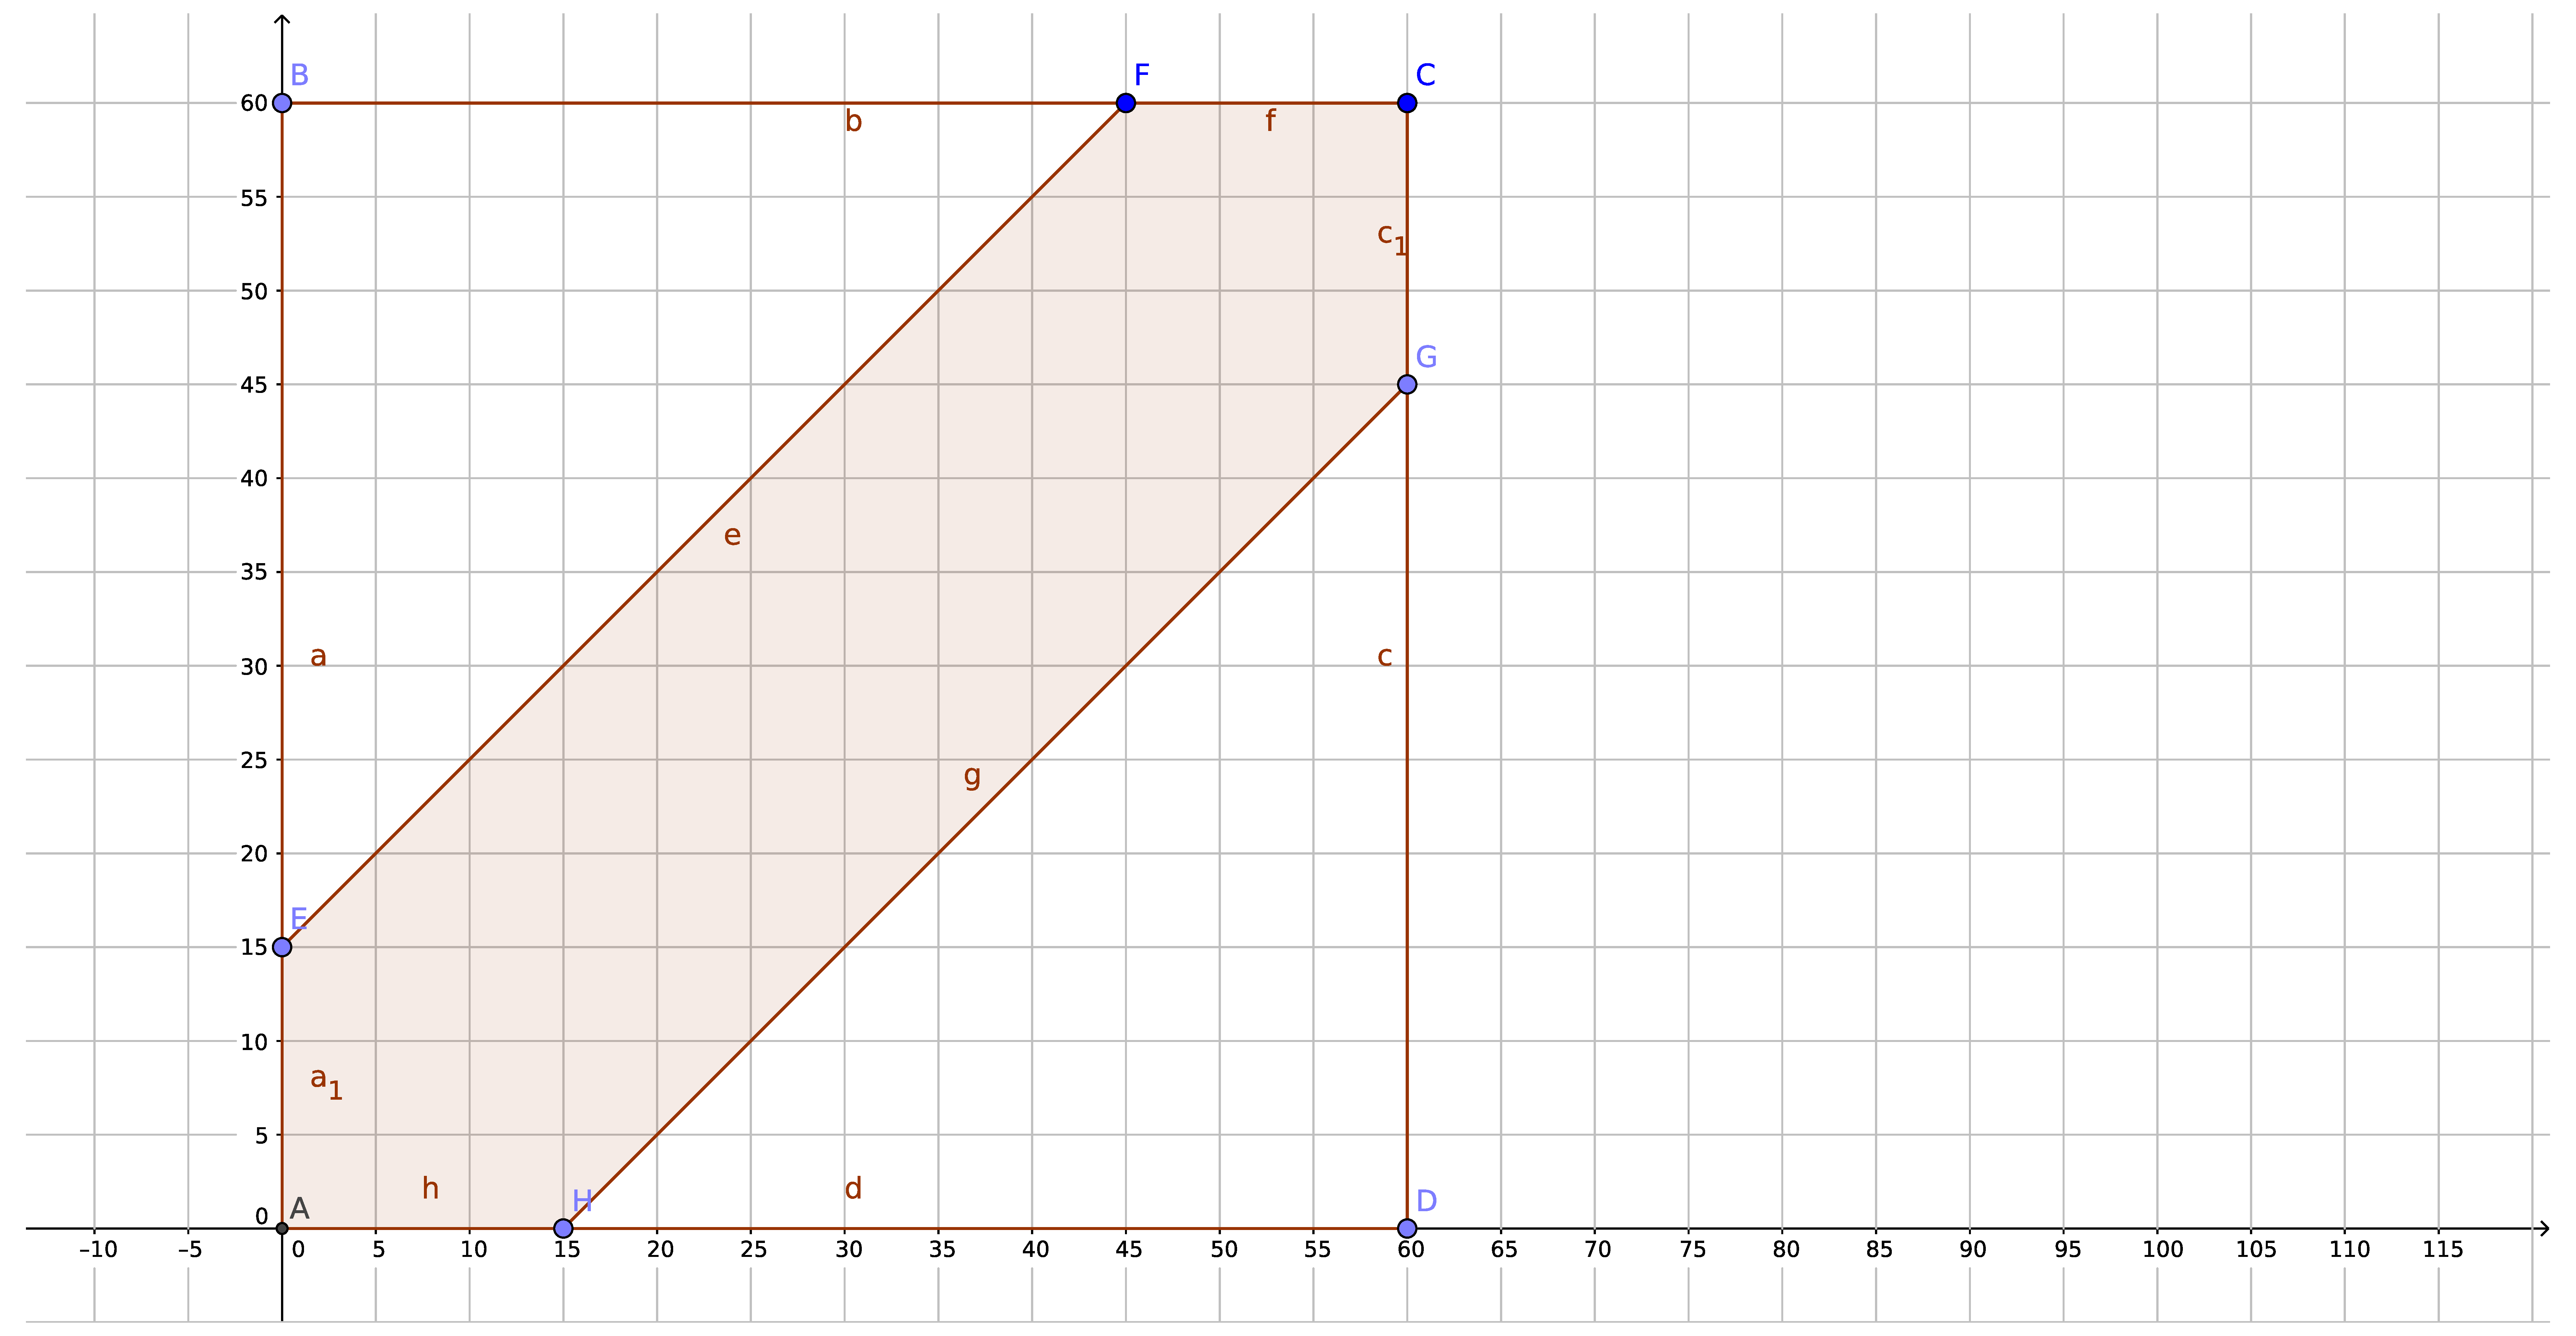
\includegraphics[width=\textwidth]{problem1.pdf}

Условие встречи: $|t_1 - t_2|\leq 15$ (попадание точки в закрашенную область)

Поэтому, $\bb P(A) = \dfr{S_{AEFCGH} }{|{\widetilde S}|} = \dfr{1575}{3600} = 0.4375$

\textbf{Ответ:} $\bb P(A) = 0.4375$

\section{}

На плоскости, замощённой одинаковыми прямоугольниками со сторонами 10 и
20 (прямоугольники примыкают сторонами), рисуют случайную окружность радиуса 4. Найдите вероятность того, что окружность имеет общие точки ровно с
тремя прямоугольниками.

\vspace{\baselineskip}

\textbf{Решение:}

\vspace{\baselineskip}

Ясно, что рассуждения можно провести в рамках одного прямоугольника. Зафиксируем центр окружности.

Условия пересечения ровно трех прямоугольников:

1) Расстояния от центра до двух ближайших сторон прямоугольника должны быть меньше 4;

2) Расстояние до ближайшей вершины прямоугольника должно быть больше 4; 

Изобразим множество, удовлетворяющее условиям.

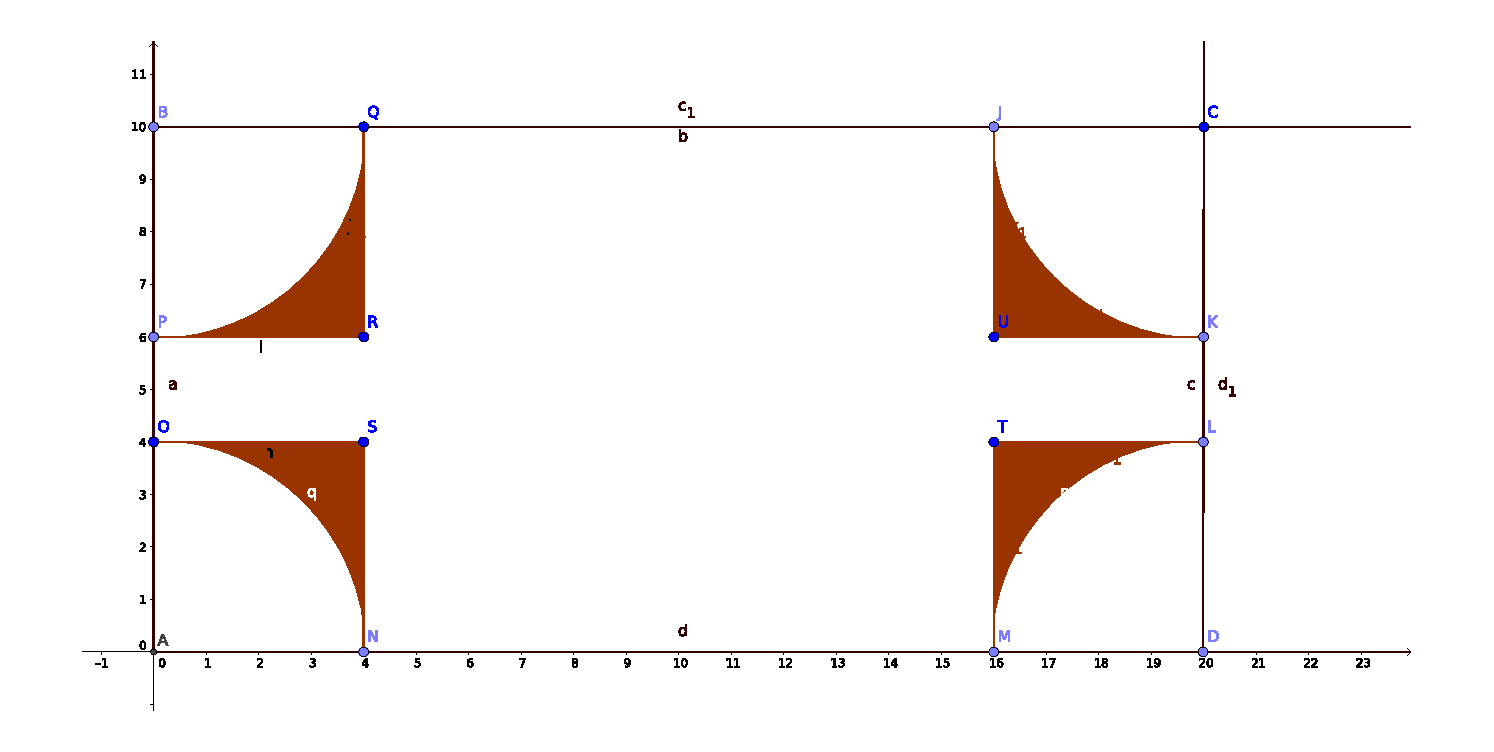
\includegraphics[width=\textwidth]{problem2.pdf}

Таким образом $\bb P = \dfr{S_{painted}}{S_{rectangle}} = \dfr{4\cdot\lt(16-\dfr{1}{4}16\pi\rt)}{10\cdot20} = \dfr{8-2\pi}{25}$

\textbf{Ответ:} $\bb P = \dfr{8-2\pi}{25}$

%3

\section{}

В тесто для выпечки булок с изюмом замешано $n$ изюмин. Всего из данного
теста выпечено $k$ булок. Оценить вероятность того, что в случайно выбранной
булке число изюмин находится в пределах от $a$ до $b$.

\vspace{\baselineskip}

\textbf{Решение:}

Пусть $X$ — число изюмин в случайно выбранной булке, с биномиальным распределением $x \in \mathbf{Bi\lt(n, \dfrac{1}{k}\rt)}$

Вероятность того,что в случано выбранной булке число изюмин равно $i$:
$$ P(i) = C^i_n  \dfrac{1}{k^i}  \lt(1- \dfrac{1}{k}\rt)^{n-i}$$

Следовательно:
$$ P(a \leq i \leq b) = \sum \limits _{i=a}^b C^i_n  \dfrac{1}{k^i} \lt(1- \dfrac{1}{k}\rt)^{n-i} = \dfrac{1}{k^n} \sum \limits _{i=a} ^b C^i_n  \lt(k-1\rt)^{n-i}$$

\vspace{\baselineskip}


\textbf{Ответ:}

%4
\section{}

Московское центральное кольцо работает с 5:45 до 1:00. Интервал движения
поездов «Ласточка» в час пик(7:30-11:30 и 16:00-21:00 в будние дни, 12:30-18:00
– в выходные) составляет 5 минут, в остальное время — 10 минут. Определить
вероятность того, что время ожидания поезда составит менее 2 минут?

\vspace{\baselineskip}

\textbf{Решение:}

\vspace{\baselineskip}

Введем следующие события:

$C =$ \{ожидание меньше 2 мин\}

$A =$ \{час пик\} $\Rightarrow$ $\ol A =$ \{не час пик\}

$D =$ \{будний день\} $\Rightarrow$ $\ol B =$\{выходной день\}

Тогда надо найти:

$\bb P(C) = \bb P(C\om) = \bb P(CA) + \bb P(C\ol A) = \bb P(CAD) +\bb P(CA\ol D) + \bb P(C\ol A D) +\bb P(C\ol A \ol D) $

Где каждый из сомножителей найдем из геометрической вероятности.

Пусть $\tau$ - время ожидания.

$t$ - время суток.

Из условия имеем:

\[
\tau = \left\{
\begin{aligned}
5,& \quad t\in \text{[7:30,11:30]}\cup \text{[16:00,21:00] в будние,} \text{[12:30,18:00] в выходные}\\
10,&\quad t\in \text{[5:45,7:30]}\cup \text{[11:30,16:00]}\cup \text{[21:00,01:00] будние,} \text{[5:45,12:30]}\cup \text{[18:00,01:00] в выходные}
\end{aligned}
\right.
\]

Время работы метрополитена - $19.25$ часов в сутки.

Поезда ходят с интервалом 5 или 10 мин.

Пассажир ожидает меньше 2 мин - множество благоприятных исходов есть последние 2 мин каждого интервала.

\vspace{\baselineskip}

$\bf CAD$ - час пик,будни

Множество благоприятных исходов есть последние 2 мин каждого 2 минутного интервала. $\Rightarrow \dfr{2}{5}$ от $\text{[7:30,11:30]}\cup \text{[16:00,21:00]} \Rightarrow \dfr{2}{5}$ от 9 часов

$$\bb P(CAD) = \fr{9}{19.25}\cdot\fr{2}{5}$$

$\bf CA\ol D$ - час пик,выходные

Множество благоприятных исходов: $\dfr{2}{5}$ от $\text{[12:30,18:00]} \Rightarrow \dfr{2}{5}$ от 5.5 часов

$$\bb P(CA\ol D) = \fr{5.5}{19.25}\cdot\fr{2}{5}$$

\vspace{\baselineskip}

$\bf C\ol AD$ - не час пик,будние

Множество благоприятных исходов: $\dfr{2}{10}$ от $\text{[5:45,7:30]}\cup \text{[11:30,16:00]}\cup \text{[21:00,01:00]} \Rightarrow \dfr{2}{10}$ от 10.25 часов

$$\bb P(C\ol AD) = \fr{10.25}{19.25}\cdot\fr{2}{10}$$

\vspace{\baselineskip}

$\bf C\ol A \ol D$ - не час пик, выходные

Множество благоприятных исходов: $\dfr{2}{10}$ от $\text{[5:45,12:30]}\cup \text{[18:00,01:00]} \Rightarrow \dfr{2}{10}$ от 13.75 часов

$$\bb P(C\ol AD) = \fr{13.75}{19.25}\cdot\fr{2}{10}$$

\vspace{\baselineskip}

Итого:
\begin{multline}
\bb P(C) = \bb P(CAD) +\bb P(CA\ol D) + \bb P(C\ol A D) +\bb P(C\ol A \ol D)=\\=
\fr{9}{19.25}\cdot\fr{2}{5} + \fr{5.5}{19.25}\cdot\fr{2}{5} + \fr{13.75}{19.25}\cdot\fr{2}{10}+ \fr{10.25}{19.25}\cdot\fr{2}{10} = 0.55 
\end{multline}

\textbf{Ответ:} $\bb P(C) = 0.55$



\end{document} % конец документа

